\begingroup
\begin{center}
\fontsize{15}{15}\sffamily\selectfont
\textbf{Trigonometric Functions}
\end{center}
\endgroup


\begin{table}[H]
    \centering
    \begin{minipage}[t]{0.3\linewidth}
        \begin{figure}[H]
            \centering
            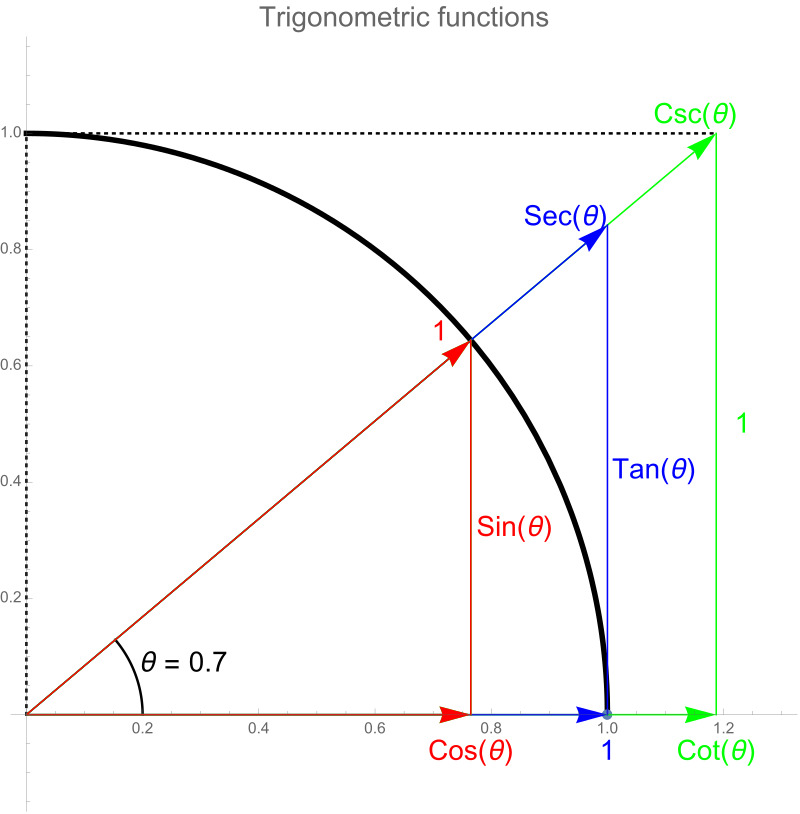
\includegraphics[height=4.5cm]{Pictures/maths/TrigFunctions.jpg}
            \caption{Trigonometry Functions Comparison}
        \end{figure}
    \end{minipage}
    \hfill
    \begin{minipage}[t]{0.3\linewidth}
        \begin{figure}[H]
            \centering
            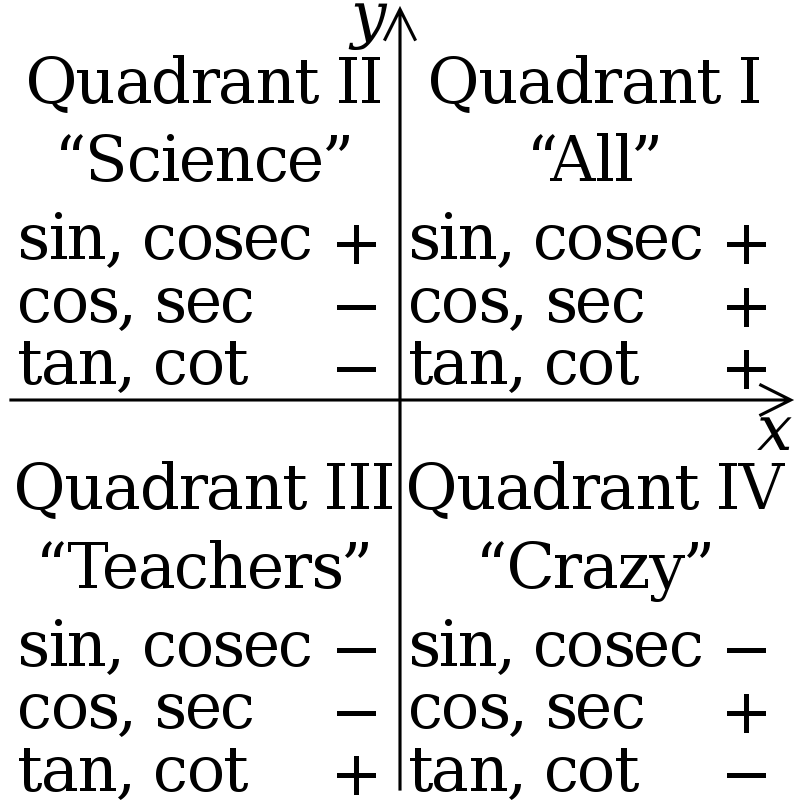
\includegraphics[height=4.5cm]{Pictures/maths/Trigonometric_function_quadrant_sign.png}
            \caption{Trigonometry Quadrant Signs}
        \end{figure}
    \end{minipage}
    \begin{minipage}[t]{0.3\linewidth}
        \begin{figure}[H]
            \centering
            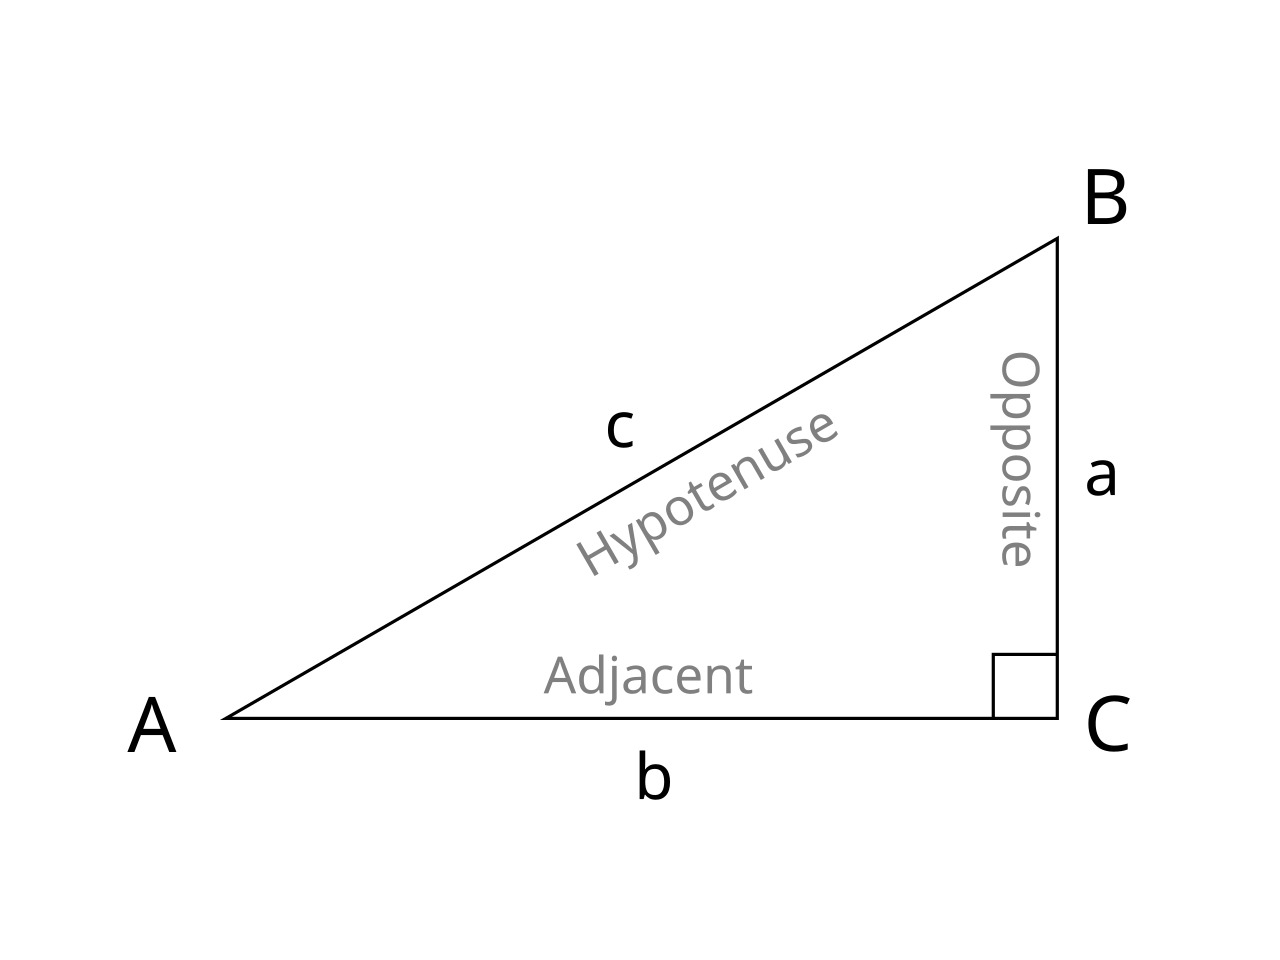
\includegraphics[height=4.5cm]{Pictures/maths/TrigonometryTriangle.jpg}
            \caption{Trigonometry Triangle}
        \end{figure}        
    \end{minipage}
\end{table}

\section{sine ( $\sin(\theta)$ )}\label{sine (sin)}

\[
    \sin(\theta) = \displaystyle \dfrac{\mathrm{opposite}}{\mathrm{hypotenuse}}
\]
\[    \sin(\theta + 2k\pi) = \sin(\theta)   \]

\section{cosine ( $\cos(\theta)$ )}\label{cosine (cos)}

\[
    \cos(\theta) = \displaystyle\dfrac{\mathrm {adjacent} }{\mathrm {hypotenuse} }
\]
\[  \cos(\theta + 2k\pi ) = \cos(\theta)  \]

\section{tangent ( $\tan(\theta)$ )}\label{tangent (tan)}

\[
    \tan(\theta) =\displaystyle \dfrac {\mathrm {opposite} }{\mathrm {adjacent} }
\]
\[  \tan(\theta + k\pi ) = \tan(\theta)  \]

\section{cosecant ( $\csc(\theta)$ }\label{cosecant (csc)}
\[
    \csc(\theta) =\displaystyle\dfrac {\mathrm {hypotenuse} }{\mathrm {opposite} }
\]

\section{secant ( $\sec(\theta)$ )}\label{secant (sec)}
\[
    \sec(\theta) =\displaystyle\dfrac {\mathrm {hypotenuse} }{\mathrm {adjacent} }
\]

\section{cotangent ( $\cot(\theta)$ )}\label{cotangent (cot)}

\[
    \cot(\theta) =\displaystyle\dfrac {\mathrm {adjacent} }{\mathrm {opposite} }
\]
\[  \cot(\theta + k\pi ) = \cot(\theta)  \]


\section*{Properties \& Formulas}
\begin{enumerate}
    \item \( \sin^2(\theta) + \cos^2(\theta) = 1 \)
\end{enumerate}



